\chapter{Systems}
\label{ch:system}
\section{Introduction}
In this section, we will discuss the system setup and the implementations of our complete system including VILENS odometry, posegraph SLAM, and place recognition server for three different operating modes. First, we discuss the system setup used for collecting data. Next, the details of implementation will show how place recognition server integrated to our SLAM system under different modes: online SLAM, offline multimission SLAM map merging, and relocalization in ROS framework. Finally, we further explore the possible implementation of replacing VILENS odometry system with existing open sourced SLAM systems (e.g. FAST-LIO, LIO-SAM) to open source our pipeline of place recognition server, which is on-going future work. 

\begin{figure}[t]
  \centering
  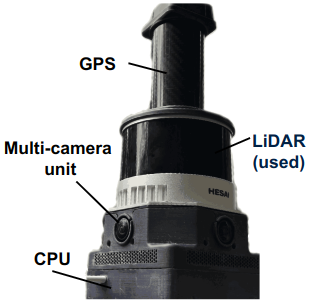
\includegraphics[width=0.4\columnwidth]{pics/setup_Frontier_pic2.png}
  \caption{Image of \emph{Frontier} comprising a LiDAR, IMU, three cameras, GPS and CPU board. }
  \label{fig:frontier}
\end{figure}

\section{Hardware Setup}
\label{sec:system_setup}
Our system uses \emph{Frontier} device as main sensors which comprises a LiDAR, IMU, and three cameras (additionally GPS) shown in \figref{fig:frontier}. We used two types of \emph{Frointers}, \emph{Frointer-15} and \emph{Frointer-19} which contains Hesai XT-32 and Hesai QT-64 LiDAR respectively and the details of sensor specifications are summarized in \tabref{tab:sensors}. For different \emph{Frontier} devices, we modify configuration settings on both VILENS and VILENS SLAM (details in \cite{wisth2023tro,proudman2022ras}). For data collection, we mainly used human and legged robot platforms as shown in \figref{fig:system_setup}. We mapped the forest area in zig-zag patterns to cover up both forward and backward views. 



\begin{table}[htbp]
  \centering
  \small
  \caption{Sensor specifications of \emph{Frontier} device.}
  \label{tab:sensors}
  \begin{tabular}{|c|c|>{\raggedright\arraybackslash}p{4.5cm}|}
      \hline
      \multicolumn{1}{|c|}{\textbf{Sensor Type}} & \multicolumn{1}{|c|}{\textbf{Name}} & \multicolumn{1}{|c|}{\textbf{Characteristics}} \\
      \hline
      \multirow{8}{*}{LiDAR} & \multirow{4}{*}{Hesai Pandar XT-32 (\emph{Frontier-15})} & \textbullet\, 10 Hz \newline \textbullet\, 360° × 31° FoV \newline \textbullet\, 0.18° × 1° Res. \newline \textbullet\, 0.5--120 m Range \\
      \cline{2-3}
      & \multirow{4}{*}{Hesai Pandar QT-64 (\emph{Frontier-19})} & \textbullet\, 10 Hz \newline \textbullet\, 360° × 104° FoV \newline \textbullet\, 0.6° × 1.45° Res. \newline \textbullet\, 0.1--60 m Range \\
      \hline
      \multirow{4}{*}{Cameras} & \multirow{4}{*}{Sevensense, Alphasense} & \textbullet\, 40 Hz \newline \textbullet\, 126° × 92.4° FoV \newline \textbullet\, RGGB Bayer \newline \textbullet\, 1440×1080 pixels \\
      \hline
      \multirow{2}{*}{IMU} & \multirow{2}{*}{Microstrain} & \textbullet\, 400 Hz \newline \textbullet\, Sync with cameras \\
      \hline
  \end{tabular}
\end{table}



\begin{figure}[t]
  \centering
  \includegraphics[width=0.80\columnwidth]{pics/setup_4yp_platform_fig3.pdf}
  \caption{Platform setup for forest mapping. Backpack (shown in left) with \emph{Frontier} mounted for a human mapping scenario, and a legged robot (shown in right) for forest surveying and monitoring applications.}
  \label{fig:system_setup}
\end{figure}


\section{Implementations}
\label{sec:implementation}
\subsection{Robotic Operating System (ROS) Framework}
The Robot Operating System (ROS) is a flexible framework for developing software for robotics applications. One of the key concepts in ROS is the publisher-subscriber model, where nodes (independent processes) communicate by publishing messages on topics and subscribing to messages on those topics. Publishers broadcast data, such as sensor readings or robot state information, while subscribers receive and process these data. The nodes and published topics then estalbish a network that represents the data sharing; this can be visualized with ROS tools such as \emph{rqt graph} in \figref{fig:implementation_ros}. Additionally, ROS facilitates communication between nodes through service calls and servers. Services allow nodes to request specific tasks or information from one another, where the client sends a request message and the server responds accordingly, enabling more complex interactions beyond simple message passing. This modular and distributed architecture of ROS makes it well-suited for building modular and scalable robotic systems. 
\begin{figure}[t]
  \centering
  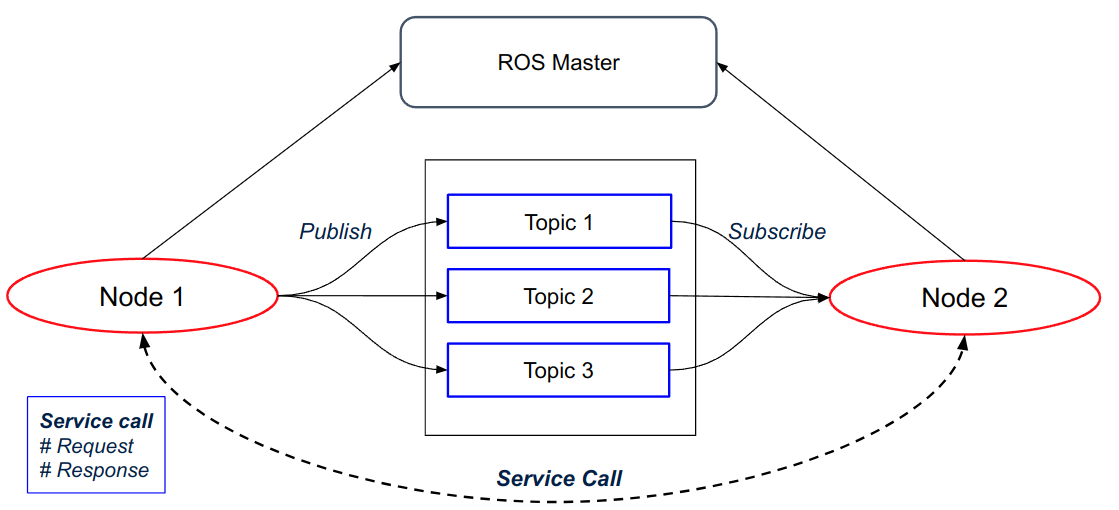
\includegraphics[width=0.8\columnwidth]{pics/Implementation_ros_framework2.png}
  \caption{ROS Framework. Nodes are shown in red elipses, published topics are shown in blue boxes. Additionally, we also define service call, a client node requests a specific service message and a server node responses a service message based on request. Edges are connections between nodes. We will follow \emph{rqt graph} convention to visualise ROS nodes and topics throughout this section.}
  \label{fig:implementation_ros}
\end{figure}

\subsection{Online SLAM}
This is a basic setup for single mission SLAM. The previous place recognition system, specifically \emph{Scan Context}, was integrated inside VILENS SLAM directly. But now, place recognition server, is integrated as a separate module and we can call different place recognition models from a new script which provides a ROS node (shown in \figref{fig:implementation_online_slam} called \emph{place recognition logg3dnet}). The place recognition server subscribes LiDAR scan and pose graph topics from VILENS SLAM. The place recognition server then publishes service messages to VILENS SLAM node. Service message contains loop candidate ids and their relative transformation. The overall online SLAM nodes and topics used are shown in \figref{fig:implementation_online_slam}. 
It works followings: When most recent LiDAR scan and posegraph are available in VILENS SLAM, place recognition node subscribes those topics and call place recnition server to extract descriptors and verify the candidates in database in \secref{ch:methods}. And then it publishes loop candidates service message back to VILENS SLAM. 

\begin{figure}[t]
  \centering
  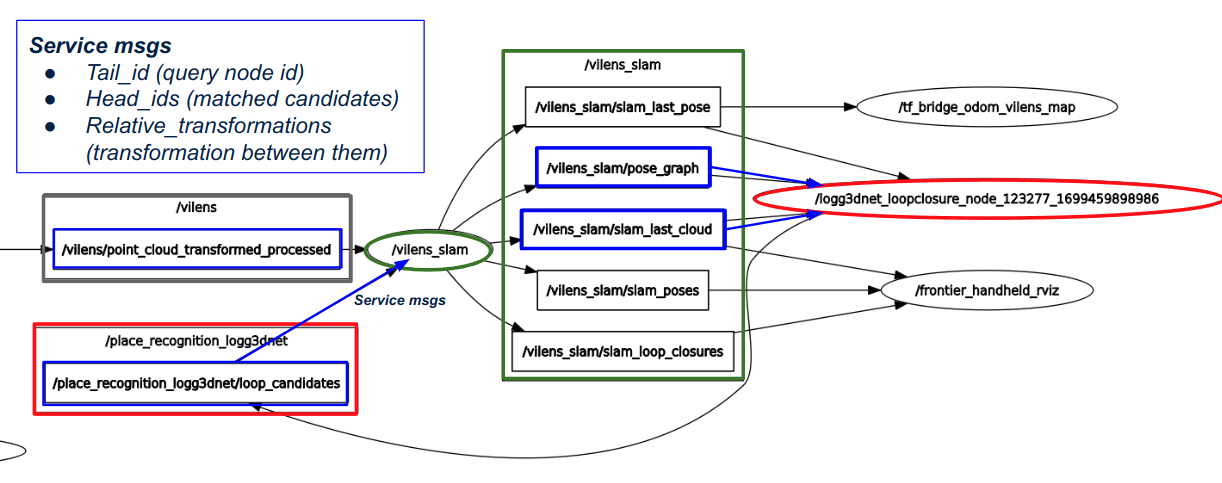
\includegraphics[width=0.99\columnwidth]{pics/Implementation_Online_SLAM2.png}
  \caption{Online SLAM Implementation (ROS rqt graph). VILENS odometry (shown in grey) and VILENS SLAM (shown in green) are our base system. The place recognition node (shown in red) subscribe topics(shown in blue) from VILENS SLAM node. Then it publishes service messages to VILENS SLAM node if loop candidates are fully verfied. Service message contains loop candidates ids and their relative transformation.}
  \label{fig:implementation_online_slam}
\end{figure}


\subsection{Offline Multi-mission SLAM Map Merging}
Offline Multi-mission SLAM maps merging is simplely done by  service call between VILENS SLAM Offline node and place recognition server node. From VILENS SLAM Offline node individual point clouds, cloud id of a mission and pose graph can be used as input to place recognition server node. The place recognition server node builds the database incrementally mission by mission. Then, when it finds loop closures it service calls back to VILENS SLAM Offline node. The overall offline multimission SLAM nodes and topics used are shown in \figref{fig:implementation_offline_slam}.  

\begin{figure}[t]
  \centering
  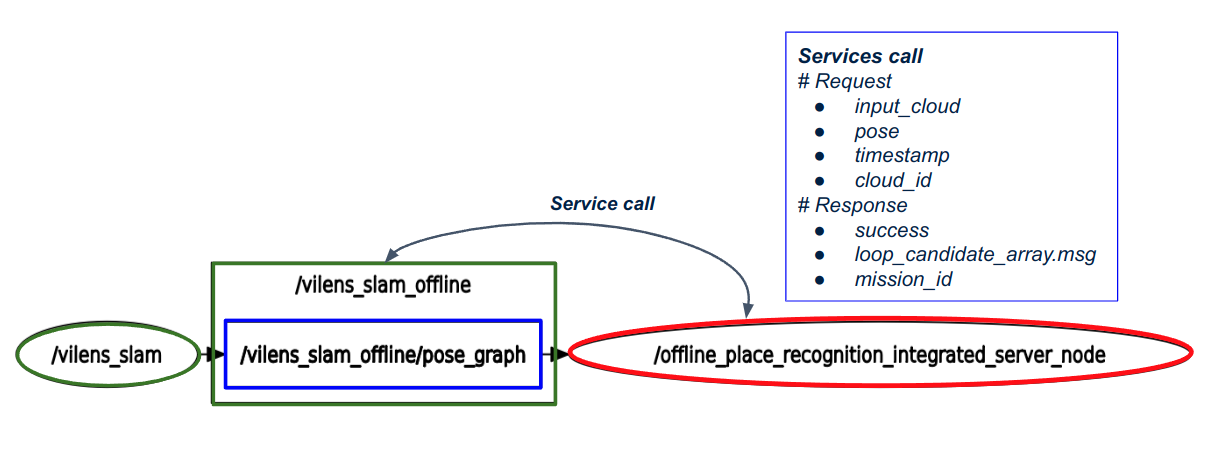
\includegraphics[width=0.99\columnwidth]{pics/Implementation_Offline_SLAM.png}
  \caption{}
  \label{fig:implementation_offline_slam}
\end{figure}


\subsection{Relocalization}
Relocalization showcases of how to use place recognition server for relocalization. As shown in \figref{fig:implementation_relocalization}, VILENS SLAM replaced by place recognition client node which stores all the prior map of individual point clouds, posegraph and descriptors. Simillar to Online SLAM mode, place recognition server node provides loop closures message to place recognition client node. The place recognition client node then relocalize the current robot's pose based on the loop closure message for visualisation. 
In order to visualise the pose of the robot continuously, we need to compute tf trees between \emph{map} and \emph{odom} shown in \figref{fig:implementation_relocalization_tf}. Once loop closures are verified from place recognition server, we can compute transformation between \emph{map} and \emph{base}. Then from VILENS odometry, we access tf between \emph{base} and \emph{odom}. Then we compute transformation between \emph{map} and \emph{base} then publish as tf messange. Now this verified tf is synchronised with VILENS odometry to visualise the pose of the robot. Anytime new loop closures are verified, we change current tf between \emph{map} and \emph{odom} and republish as tf message. 

Lastly, we implemented virtual rendering of tree models using OpenGL (GPU accelerated) library for real-time visualisation of both camera images and virtual tree models. 
\begin{figure}[t]
  \centering
  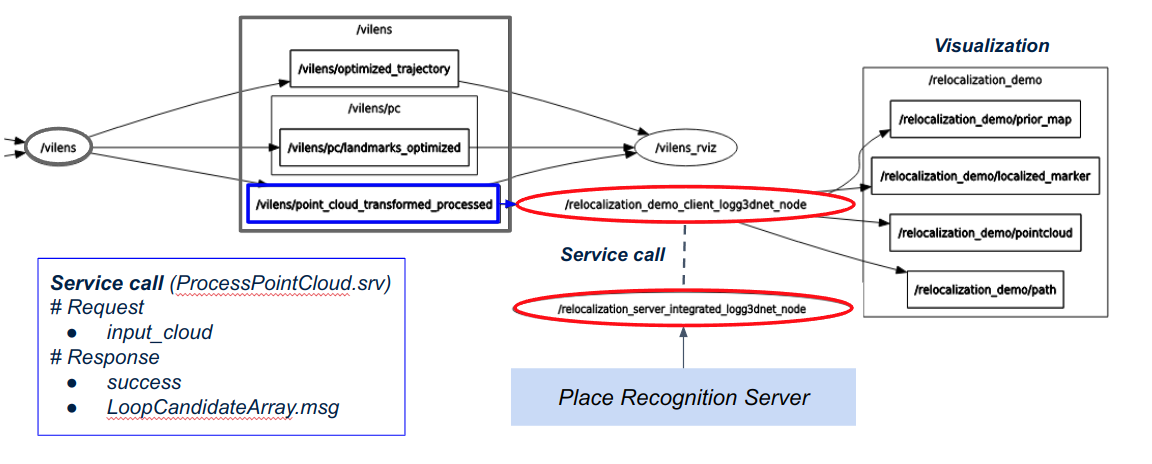
\includegraphics[width=0.99\columnwidth]{pics/Implementation_Relocalization1.png}
  \caption{Relocalization (ROS rqt graph). Relocalization demonstrates a }
  \label{fig:implementation_relocalization}
\end{figure}



\begin{figure}[t]
  \centering
  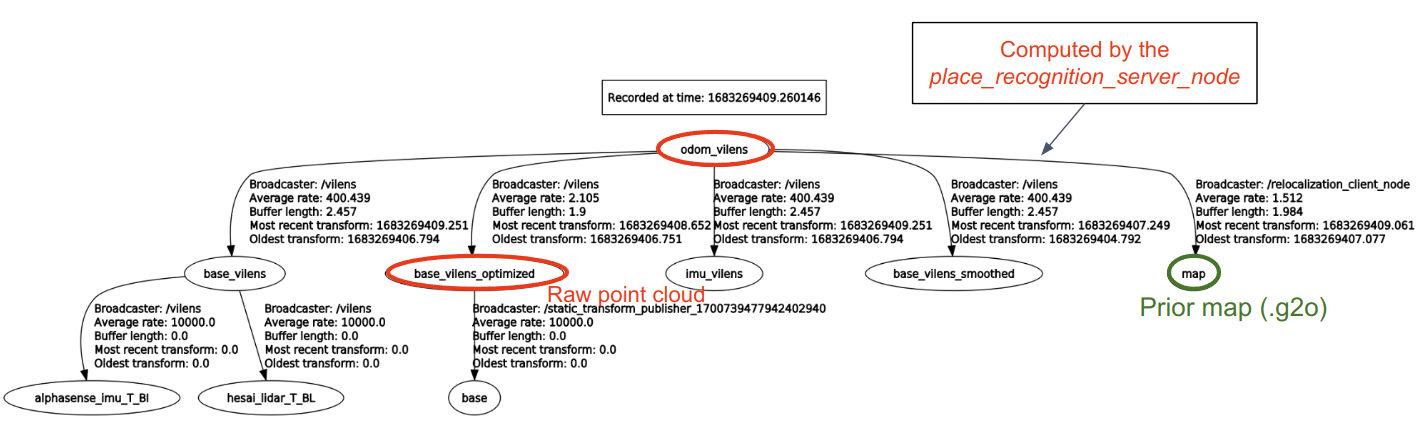
\includegraphics[width=0.99\columnwidth]{pics/impelementation_relocalization_tf.png}
  \caption{Tf tree for relocalization. Tf between \emph{map} and \emph{odom} should be connected from place recognition server node.}
  \label{fig:implementation_relocalization_tf}
\end{figure}